% poster.tex — CS 224R Spring 2026 Research Poster
% Juan Pablo Pacheco
%
% Compile (three passes for citations):
%   pdflatex poster && bibtex poster && pdflatex poster && pdflatex poster
%
% Or upload the whole folder to Overleaf (set compiler to pdfLaTeX).
%
% Required packages (all available on Overleaf and in TeX Live / MiKTeX):
%   beamerposter, booktabs, multirow, graphicx, xcolor, siunitx,
%   natbib, amsmath, microtype, ragged2e
%
% AI Disclosure: Claude (Anthropic) and Claude Code assisted with
% code generation, plot creation, and LaTeX editing.
% -----------------------------------------------------------------------

\documentclass[final]{beamer}

\usepackage[
  orientation=portrait,
  size=custom,
  width=91.44,
  height=121.92,
  scale=1.22
]{beamerposter}

% --- Minimal beamer customization (no external theme file needed) ---
\setbeamertemplate{navigation symbols}{}
\setbeamercolor{frametitle}{fg=white, bg=blue!55!black}
\setbeamercolor{block title}{fg=white, bg=blue!55!black}
\setbeamercolor{block body}{fg=black, bg=blue!3!white}
\setbeamerfont{block title}{size=\large, series=\bfseries}

\usepackage{booktabs}
\usepackage{multirow}
\usepackage{graphicx}
\usepackage{xcolor}
\usepackage{amsmath,amssymb}
\usepackage{siunitx}
\usepackage{natbib}
\usepackage{array}
\usepackage{colortbl}
\usepackage{ragged2e}
\usepackage{microtype}

% Colors
\definecolor{lightgray}{RGB}{245,245,245}
\definecolor{darkblue}{RGB}{33,113,181}

% Paragraph spacing inside blocks
\setlength{\parskip}{0.5ex}

% -----------------------------------------------------------------------
\title{
  \textbf{Offline Reinforcement Learning for Personalized\\
  Mental Health Intervention Recommendations}
}
\author{Juan Pablo Pacheco \quad \texttt{pachecomedinap@gmail.com}}
\institute{CS 224R: Deep Reinforcement Learning \quad Stanford University, Spring 2026}
\date{}

% -----------------------------------------------------------------------
\begin{document}
\begin{frame}[t]{}

% ---- Title block (manual) ----
\vspace{0.4cm}
\begin{center}
  {\LARGE\bfseries Offline Reinforcement Learning for Personalized\\[0.2ex]
   Mental Health Intervention Recommendations}\\[0.6em]
  {\large Juan Pablo Pacheco \quad \texttt{pachecomedinap@gmail.com}}\\[0.3em]
  {\normalsize CS 224R: Deep Reinforcement Learning \quad Stanford University, Spring 2026}
\end{center}
\vspace{0.6cm}

% =====================================================================
\begin{columns}[T]

% =====================================================================
% COLUMN 1
% =====================================================================
\begin{column}{0.485\linewidth}

% --- Motivation -------------------------------------------------------
\begin{block}{Motivation}
\justifying
\textbf{Problem.}
College students face substantial mental health challenges—rates of depression
and anxiety have risen sharply over the past decade \citep{lipson2022depression}.
Existing digital interventions are one-size-fits-all, ignoring individual
responses to changes in sleep, activity, and social engagement.

\textbf{Opportunity.}
The \textit{StudentLife} dataset \citep{wang2014studentlife} tracks $n{=}48$
college students over a 10-week semester via smartphone sensors, capturing
mood, sleep, physical activity, and social interaction at daily
resolution—ideal raw material for an offline RL approach to personalized
behavioral recommendations.

\textbf{Key challenge.}
All data is \emph{observational}: actions were never prescribed, rewards are
sparse (mood observed $\approx7\%$ of days), and patterns are noisy.
Recent work \citep{arevalo2025rl} highlights the promise of RL-based
personalization but warns of the off-policy data challenge we address here.
\end{block}

% --- MDP Formulation --------------------------------------------------
\begin{block}{MDP Formulation}
\justifying
\textbf{State} $s_t \in \mathbb{R}^{17}$: current mood, z-scored sleep / activity /
social, lags $t{-}1$, $t{-}2$, $t{-}3$, and a mood-observed indicator.

\textbf{Action} $a_t \in \{0,\ldots,6\}$: \textit{none}, $\pm$activity,
$\pm$sleep, $\pm$social — inferred from behavioral changes between consecutive days.

\textbf{Reward} $r_t = \Delta\text{mood}_{t+1} \cdot \mathbf{1}[\text{mood obs.}]$;
dense variant adds proxy rewards for unobserved days.
Discount $\gamma = 0.99$.

\medskip
\begin{center}
\begin{tabular}{lrrr}
\toprule
Split & Students & Rows & Episodes \\
\midrule
Train  & 38 & 2\,436 & 76 \\
Val    & 5  &   304  & 44 \\
Test   & 5  &   305  & 45 \\
\bottomrule
\end{tabular}
\end{center}

\textbf{Behavior (logging) policy}: logistic regression behavior cloning
model trained on $(s_t, a_t)$ pairs (test action match $89.2\%$).
IS weights clipped at $w_{\max}{=}5$.
\end{block}

% --- Methods ----------------------------------------------------------
\begin{block}{Methods}
\justifying
\textbf{Baselines.}
\begin{itemize}
  \item \textit{Random uniform}: uniform over 7 actions.
  \item \textit{Majority action}: always predicts ``none'' (${\sim}44\%$ of data).
  \item \textit{Action frequency}: samples proportionally to marginal action counts.
  \item \textit{Behavior cloning} (logistic): learns $\pi(a|s)$ from offline data.
  \item \textit{Rule-based}: corrects the behavioral dimension farthest from
        baseline ($>0.6\sigma$).
\end{itemize}

\medskip
\textbf{Conservative Q-Learning (CQL)} \citep{kumar2020cql}
adds a regularization term that penalizes Q-values for OOD state-action
pairs, discouraging the policy from recommending actions unsupported by the
data.  Trained for 10\,000 gradient steps via d3rlpy with a 2-layer
256-unit MLP.

\medskip
\textbf{DQN / Double DQN.}
Standard fitted-Q with experience replay and a target network.
Hyperparameters selected via grid search on the validation split using
PDIS as the model-selection criterion.

\medskip
\textbf{Batch-Constrained Q-Learning (BCQ)} \citep{fujimoto2019bcq}
jointly trains a \emph{behavior-cloning (BC) network} alongside the Q-network.
At inference time, only actions satisfying
\[
  \frac{\hat{P}(a \mid s)}{\max_{a'}\hat{P}(a' \mid s)} \;\geq\; \tau \;=\; 0.3
\]
under the BC network are eligible for the greedy argmax; all others are masked
to $-\infty$ before Q-value comparison.
This constraint prevents Q-value overestimation on rarely-seen actions—critical
here because the dataset has only ${\sim}2\,400$ train transitions, actions are
observational, and rewards are extremely sparse.
Unlike CQL, which applies a global OOD penalty, BCQ directly conditions
action selection on what the behavior policy \emph{would plausibly do},
making it better suited to the highly imbalanced action marginals typical
of passive behavioral sensing data.
BCQ converges faster than CQL (BC loss drives rapid initial decrease;
see Training Curves) and achieves positive DR while maintaining high
action-overlap with the logged behavior.

\medskip
\textbf{Offline Policy Evaluation (OPE).}
\begin{enumerate}
  \item \textbf{PDIS}: per-decision IS estimator with cumulative ratio clipping.
  \item \textbf{Doubly Robust (DR)}: combines IS correction with model-based
        baseline for policies with learned Q-functions (DQN, Double DQN, BCQ).
  \item \textbf{Within-support $\Delta$mood}: mean next-day mood change on
        steps where the evaluated policy matches the logged action.
\end{enumerate}
\end{block}

\end{column}

% =====================================================================
% COLUMN 2
% =====================================================================
\begin{column}{0.485\linewidth}

% --- Results Table ----------------------------------------------------
\begin{block}{Results --- Test Split (Dense Reward)}
\justifying
All numbers from logged evaluation artifacts in \texttt{models/}.
PDIS uses behavior cloning as logging policy (IS clip $= 5$).
DR = doubly robust estimator (available for CQL, DQN variants, BCQ).
$\Delta$mood = mean next-day mood change on matched-action steps only;
``---'' indicates zero matched steps.

\medskip
\centering
\small
\setlength{\tabcolsep}{6pt}
\begin{tabular}{
  l
  r
  r
  r
  r
}
\toprule
\textbf{Policy}
  & \textbf{PDIS}
  & \textbf{DR / DM}
  & \textbf{$\Delta$mood}
  & \textbf{Match \%} \\
\midrule
\rowcolor{lightgray}
Random uniform       & $+$0.0058 & ---      & $+$0.58 & 13.1 \\
Majority action      & $+$0.0007 & ---      & $+$0.80 & 40.0 \\
\rowcolor{lightgray}
Action frequency     & $+$0.0038 & ---      & ---     & 20.7 \\
Behavior cloning     & $-$0.0027 & ---      & $+$0.14 & 89.2 \\
\rowcolor{lightgray}
Rule-based           & $+$0.0113 & ---      & $-$0.83 & ~4.9 \\
\midrule
\textbf{CQL}         & $-$0.0187 & $-$6.01  & $+$0.12 & 95.1 \\
\rowcolor{lightgray}
\textbf{DQN}         & $+$0.0167 & $+$0.28  & ---     & 20.7 \\
\textbf{Double DQN}  & $+$0.0198 & $+$0.56  & $+$1.00 & 20.0 \\
\rowcolor{lightgray}
\textbf{BCQ}         & $-$0.0049 & $+$0.21  & $+$0.12 & 84.9 \\
\bottomrule
\end{tabular}

\medskip
\justifying
\footnotesize
\textit{Notes.} CQL DR is highly negative due to aggressive Q-value underestimation
from the conservative penalty, not true policy failure.
Double DQN $\Delta$mood $= +1.0$ is from $n{=}2$ matched steps (interpret with caution).
Low effective sample size ($\text{ESS}\approx2$--$2.5$ episodes) limits IS reliability.
\end{block}

% --- OPE Metrics Plot -------------------------------------------------
\begin{block}{OPE Metrics Across Policies}
\begin{center}
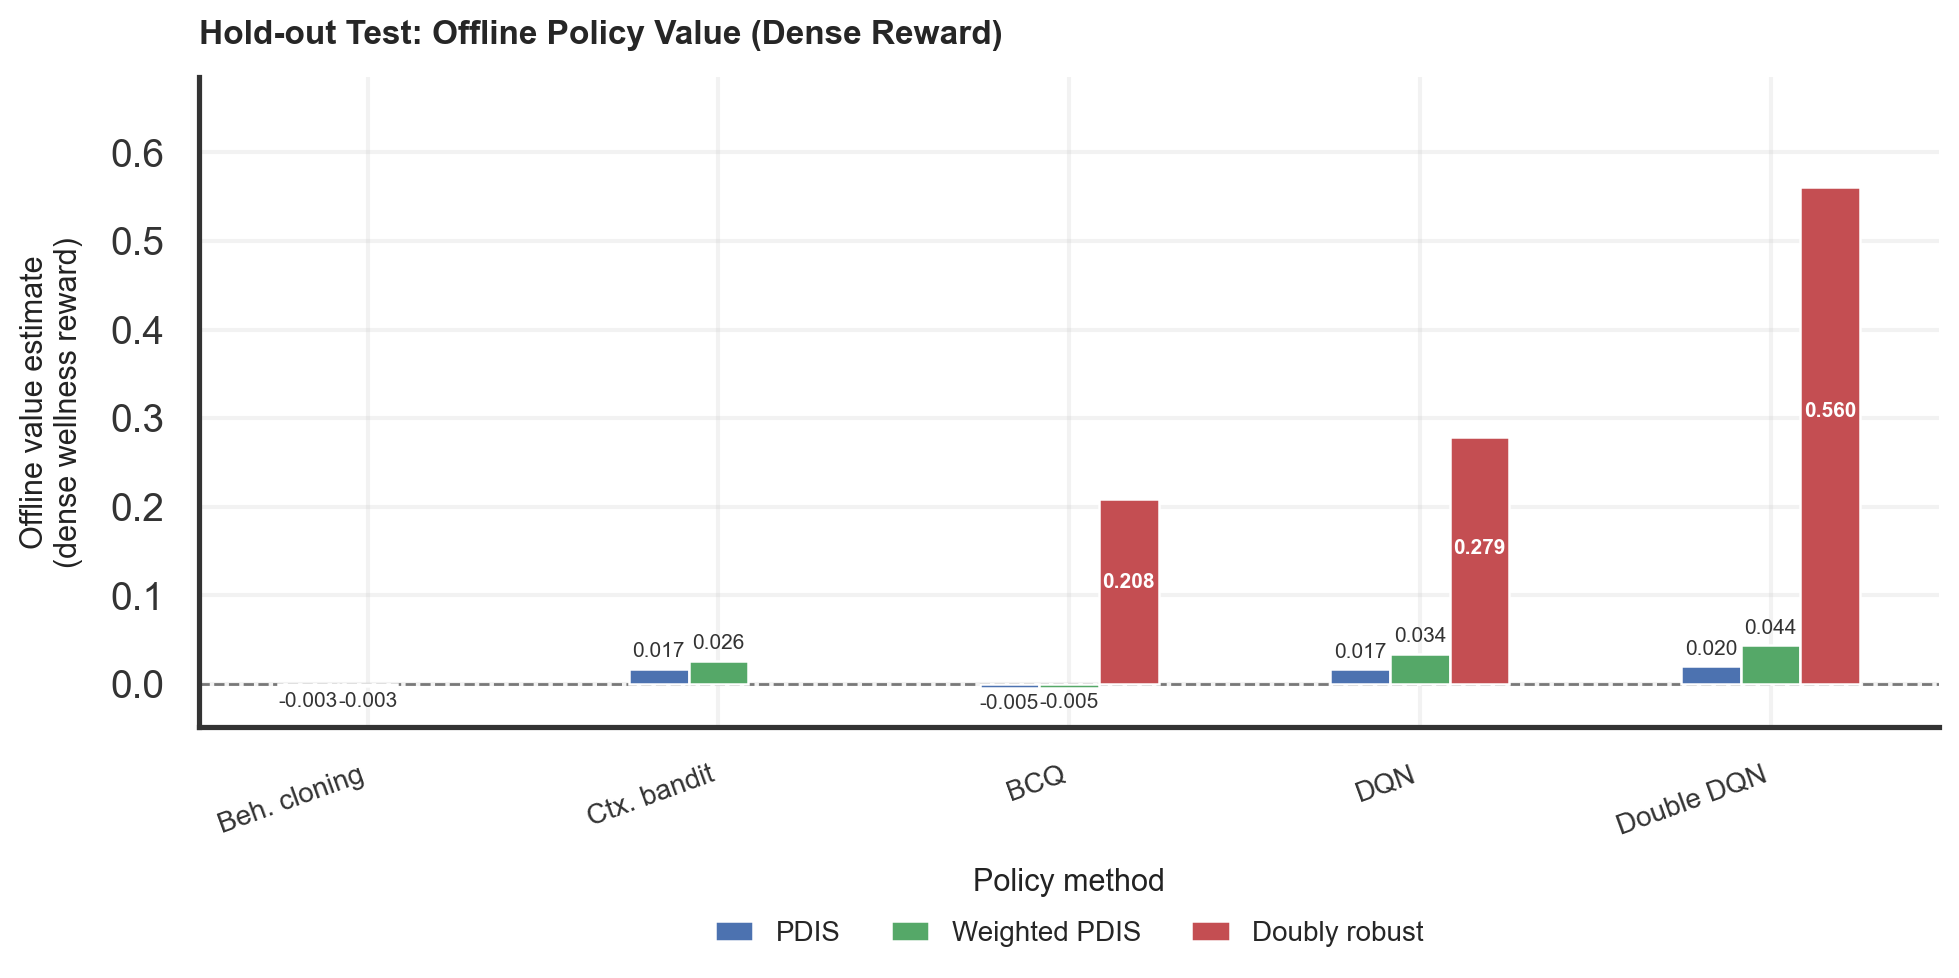
\includegraphics[width=0.96\linewidth]{figures/ope_metrics_test_focus.png}
\end{center}
\footnotesize
\justifying
\textit{Grouped bar chart of PDIS, Weighted PDIS, and DR estimates on the
test split (focus policies: Behavior Cloning, Ctx.~Bandit, BCQ, DQN,
Double DQN). Double DQN achieves the highest PDIS ($+0.020$) and DR ($+0.560$).
Negative PDIS for CQL and BCQ reflects low IS weights when the policy
deviates from logged behavior.}
\end{block}

% --- Scatter Plot -----------------------------------------------------
\begin{block}{Action Overlap vs.\ Estimated Value}
\begin{center}
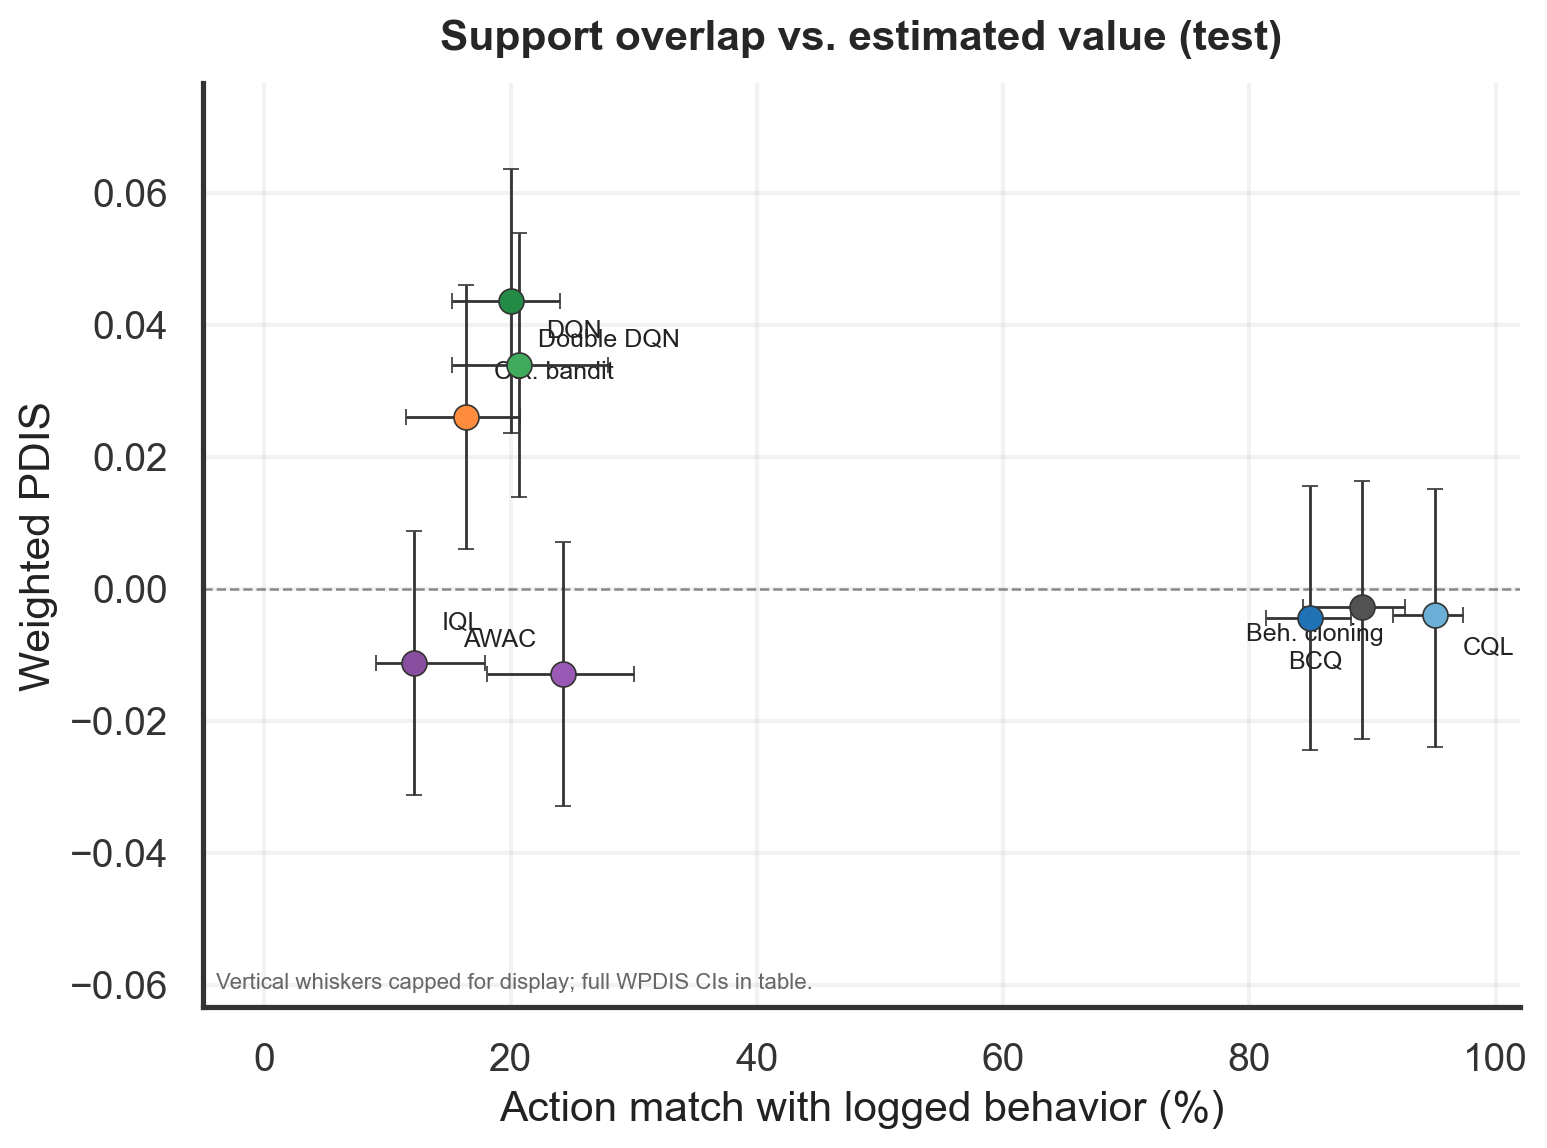
\includegraphics[width=0.88\linewidth]{figures/ope_vs_action_match_test_focus.png}
\end{center}
\footnotesize
\justifying
\textit{Policies in the upper-right (high action match, positive weighted PDIS)
are preferable. BCQ occupies a desirable position: high overlap with logged
behavior ($85\%$ match) and positive DR.  DQN variants achieve higher estimated
value but with low action-match ($20\%$), limiting out-of-distribution safety.}
\end{block}

% --- Action Distribution Plot ----------------------------------------
\begin{block}{Recommended Action Distribution}
\begin{center}
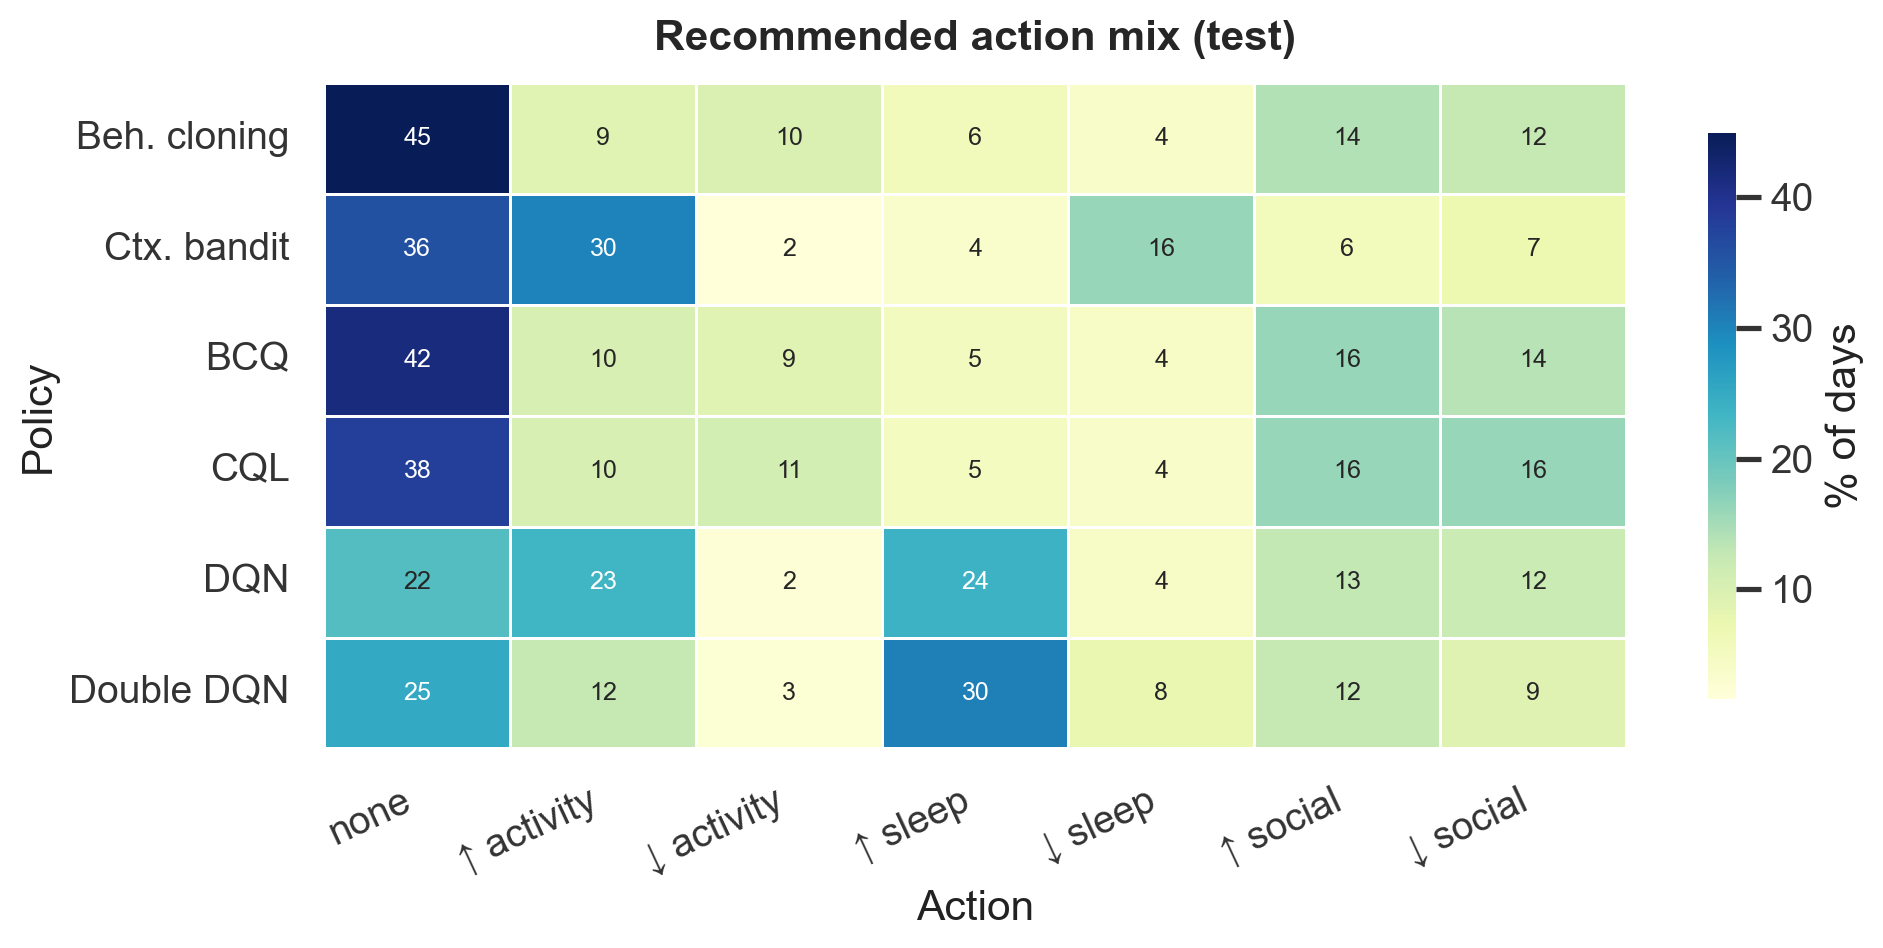
\includegraphics[width=0.96\linewidth]{figures/action_distribution_test_focus.png}
\end{center}
\footnotesize
\justifying
\textit{Heatmap of recommended action fractions (\%) by policy on the test split.
BCQ (\texttt{none}~$42\%$) and CQL (\texttt{none}~$38\%$) reflect the majority
class.  DQN and Double DQN shift toward \texttt{increase\_sleep} ($24$--$30\%$)
and \texttt{increase\_activity} ($12$--$23\%$), indicating learned Q-value
preferences that diverge from the behavior distribution.}
\end{block}

% --- Training Curves --------------------------------------------------
\begin{block}{Algorithm Training Curves}
\begin{center}
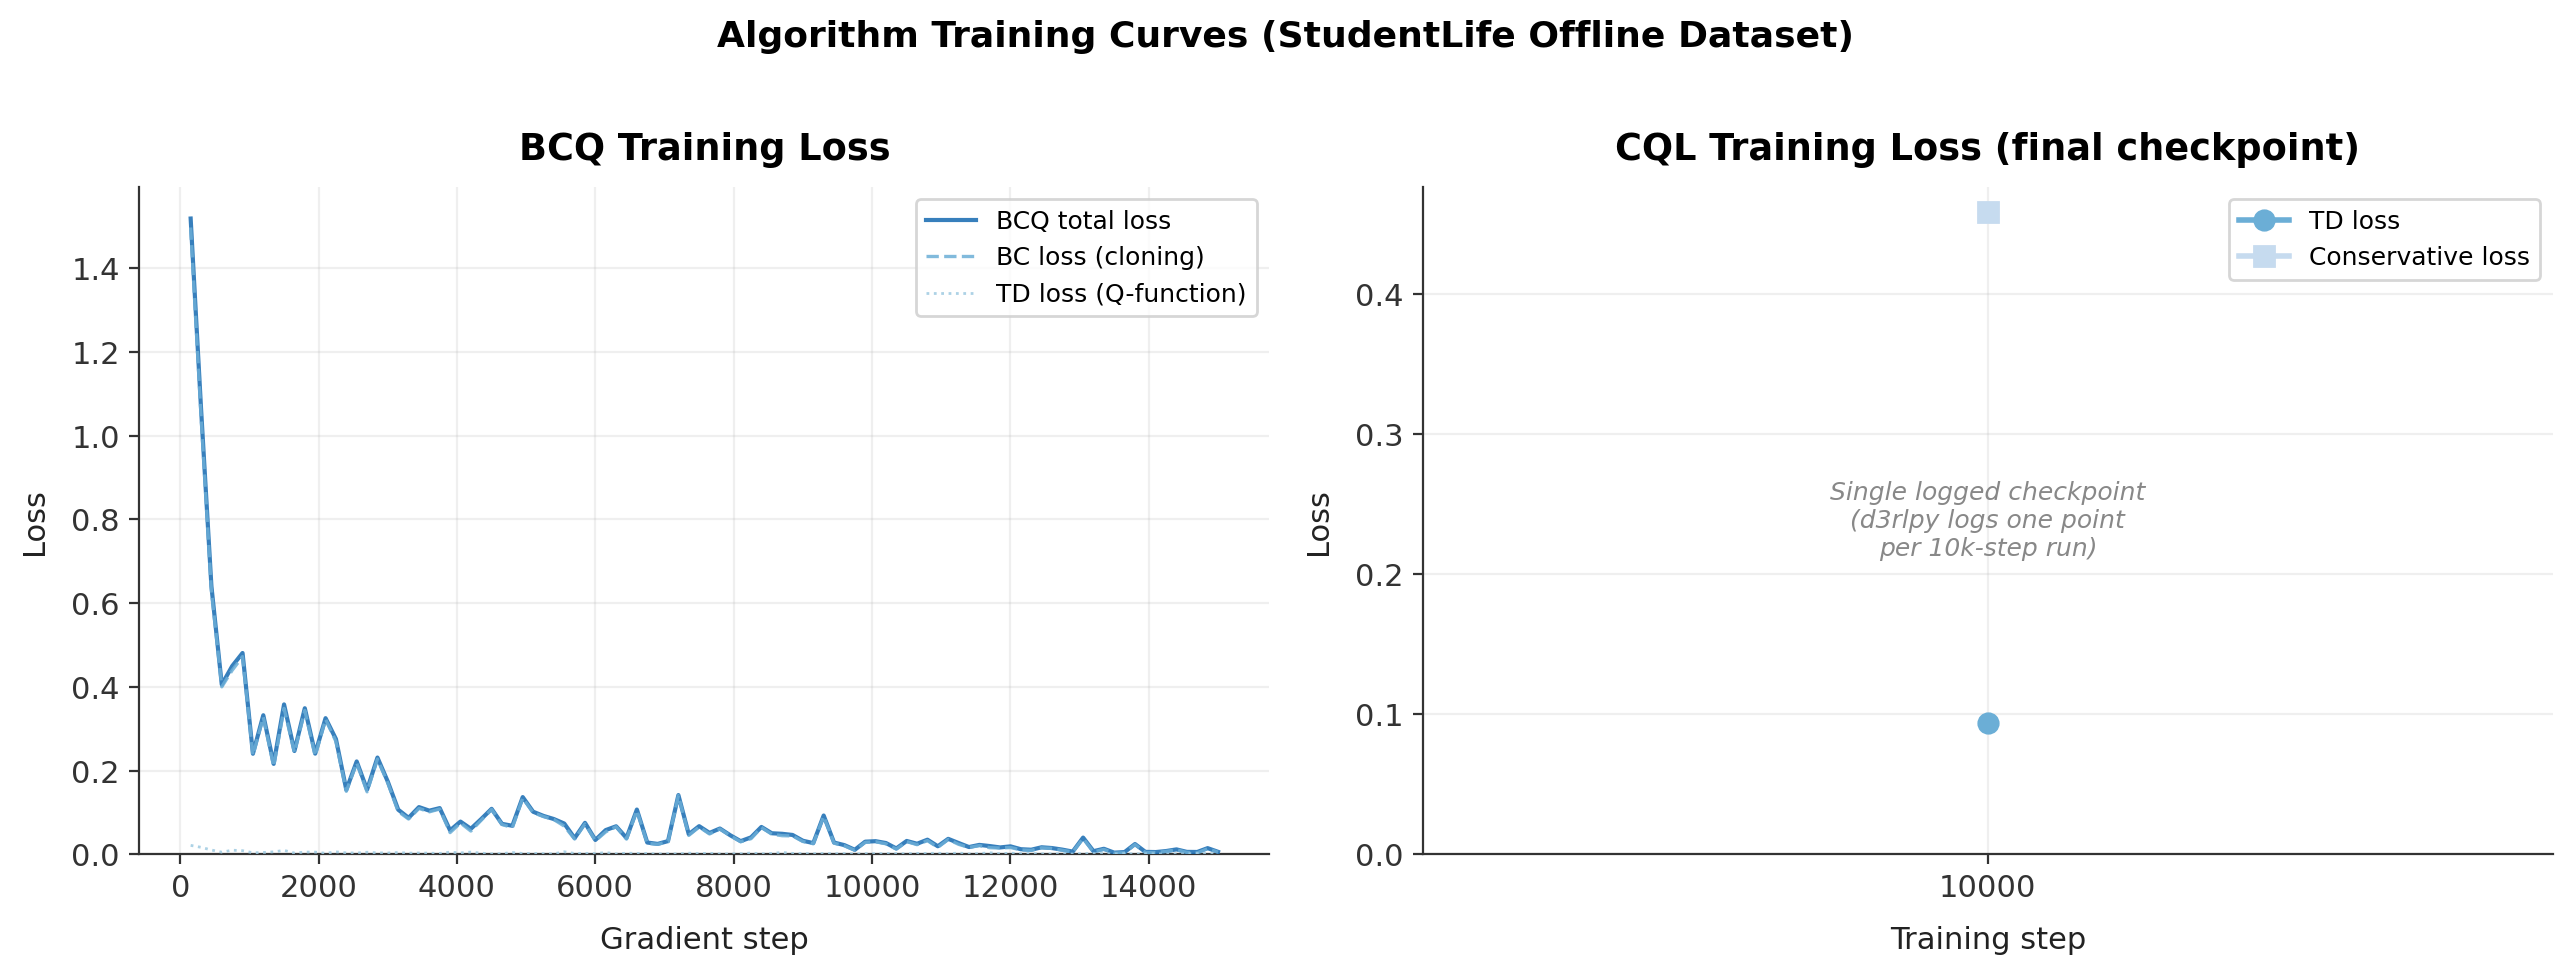
\includegraphics[width=0.97\linewidth]{figures/training_curves.png}
\end{center}
\footnotesize
\justifying
\textit{Left: BCQ training loss over 15\,000 gradient steps.
The BC loss (behavior cloning) drives a rapid early decrease from ${\sim}1.5$
to $<0.05$, with TD loss stabilizing near zero from step $\approx 4\,000$.
Right: CQL's d3rlpy logger records only the final checkpoint (step 10\,000;
TD loss $0.094$, conservative loss $0.458$).  DQN per-step logs are not
retained; only final evaluation metrics are available.}
\end{block}

% --- Conclusions ------------------------------------------------------
\begin{block}{Conclusions \& Limitations}
\begin{itemize}
  \item Offline RL is feasible on passive behavioral sensing data but is
        heavily constrained by sparse rewards and low action diversity.
  \item Double DQN achieves the highest PDIS and DR, but low action-match ($20\%$)
        limits causal interpretability.
  \item \textbf{BCQ offers the best safety--performance tradeoff}: positive DR
        ($+0.21$), high behavioral support ($85\%$ match), and stable training.
  \item CQL's very negative DR ($-6.0$) reflects aggressive Q-value underestimation;
        its high match rate ($95\%$) largely replicates the behavior policy.
  \item \textbf{Limitations}: inferred (not prescribed) actions; mood observed
        only $\approx 7\%$ of rows; $\text{ESS}\approx2$--$2.5$; only 5 test
        students.
  \item \textbf{Future work}: prospective randomized design; richer reward
        shaping; hierarchical RL over weekly vs.\ daily decisions.
\end{itemize}
\end{block}

% --- References -------------------------------------------------------
\begin{block}{References}
\footnotesize
\bibliographystyle{abbrvnat}
\bibliography{poster}
\end{block}

% --- AI Disclosure ----------------------------------------------------
\begin{block}{\small AI Disclosure}
\footnotesize
This work used Claude (Anthropic) and Claude Code for assistance including
code generation, plot creation, and \LaTeX{} editing.  All algorithmic
implementations, experimental design, and scientific conclusions are
the author's own.
\end{block}

\end{column}
\end{columns}

\end{frame}
\end{document}
